% Created 2016-06-10 Fri 13:39
\documentclass[12pt,t,xcolor=table]{beamer}

\input{/home/stephan/H/Styles/style_presentation.tex}
\usetheme{default}
\author{Stephan Lindner}
\date{6/7/2016}
\title{Exacloud: An Overview}
\begin{document}

\maketitle

\section{What is Exacloud? And why is it on a Linux server?}
\label{sec:orgheadline5}
\begin{frame}[c]{}
  \begin{itemize}
    \item[\bf\thesection.] \bf\insertsection
  \end{itemize}          
\end{frame}

\begin{frame}[label={sec:orgheadline1}]{What is Exacloud?}
\begin{itemize}
\item Exacloud a server run by OHSU to support large-scale, computational and data intense workflows.

\item Currently more than 35 Terabytes of memory and more than 750 Terabytes of usable storage.

\item Housed at the Data Center at OHSU's West Campus.
\end{itemize}

\vspace{1em}
\begin{center}
  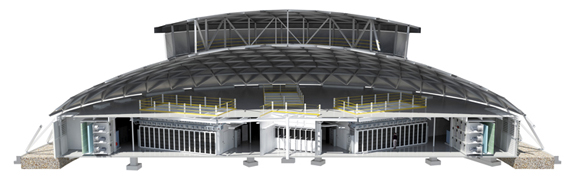
\includegraphics[width=.8\textwidth]{Figures/ohsu-datacenter.png}
\end{center}
\end{frame}


\begin{frame}[label={sec:orgheadline2}]{Exacloud and Linux}
\begin{itemize}
\item Exacloud uses Linux as operating system.

\item By contrast, the CHSE server (and our computers) use Windows as operating systems.

\item An operating systems is the ``habitat of your programs'' --- the software that manages a computer's basic functioning.

\item Linux and Windows get along OK, but they do not particularly like each other.

\item Most programs (such as R, stata) are developed for both OS (and Mac's OS).
\end{itemize}
\end{frame}

\begin{frame}[label={sec:orgheadline3}]{Why does Exacloud uses Linux?}
Linux is \ldots{}

\begin{itemize}
\item Very stable.

\item Slim and scalable and therefore has less hardware requirements.

\item Designed as a multi-user system.

\item More secure than Windows.

\item FOSS (Free and Open Source Software).
\end{itemize}
\end{frame}

\begin{frame}[label={sec:orgheadline4}]{What does this mean for us:}
\begin{itemize}
\item Most programs we use for our analysis are open-source and are developed on Linux: R, git, markdown.

\item Stata is more geared toward Windows but has some Linux support.

\item Interaction between local Windows machines and a Linux server are not perfect but fine.
\end{itemize}
\end{frame}

\section{Accessing and navigating Exacloud}
\label{sec:orgheadline9}
\begin{frame}[c]{}
  \begin{itemize}
    \item[\bf\thesection.] \bf\insertsection
  \end{itemize}          
\end{frame}

\begin{frame}[label={sec:orgheadline6}]{Accessing Exacloud via ssh}
\begin{itemize}
\item Remote access of CHSE server: through Windows desktop.

\item Remote access of Exacloud: through ssh (secure shell).

\item Shell is a command prompt that you can use to interact with the computer (e.g., run programs).

\item Bare-bone, 1970 technology that requires very little memory.
\end{itemize}
\end{frame}

\begin{frame}[fragile,label={sec:orgheadline7}]{MobaXterm: ssh for Windows}
 \begin{itemize}
\item Install MobaXterm on desktop.

\item Initiate ssh session with 
\begin{itemize}
\item Remote host: \texttt{exacloud.ohsu.edu}
\item User name: your OHSU user name.
\end{itemize}

\item Prompts for password and then connects to server.
\end{itemize}


\emph{Switch to MobaXterm}
\end{frame}

\begin{frame}[fragile,label={sec:orgheadline8}]{Navigating Exacloud}
 A couple of useful commands:

\begin{itemize}
\item Printing the working directory: \texttt{pwd}

\item Listing files in current directory: \texttt{ls (-lh / -a)}

\item Start R: \texttt{R}

\item Start stata: \texttt{stata}

\item Check git status: \texttt{git status}

\item Work with hcondor (?): \texttt{condor\_submit}, \texttt{condor\_q}
\end{itemize}
\end{frame}
\section{Interactive and non-interactive use of Exacloud}
\label{sec:orgheadline17}
\begin{frame}[c]{}
  \begin{itemize}
    \item[\bf\thesection.] \bf\insertsection
  \end{itemize}          
\end{frame}

\begin{frame}[label={sec:orgheadline10}]{Interactive versus non-interactive R / Stata session:}
\begin{enumerate}
\item Interactive: 

\begin{itemize}
\item Workflow: Work on code in script file --> Evaluate code in R / Stata --> Revise / Debug code --> \ldots{}

\item Setup: Umbrella program that integrates editor with statistical program: RStudio, standard Stata GUI, etc.

\item Requirement: Umbrella program needs to be able to transfer code chunks to Stata / R and display results.
\end{itemize}

\item Non-interactive mode:

\begin{itemize}
\item Workflow: Write full script file --> run full script in R / Stata --> Revise / Debug --> \ldots{}

\item Setup: Call script file through umbrella program / shell.

\item Requirements: some way to call R / Stata.
\end{itemize}
\end{enumerate}
\end{frame}

\begin{frame}[label={sec:orgheadline11}]{Interactive mode on servers:}
Two different options:

\begin{enumerate}
\item Run umbrella program and R / Stata on server:

\begin{itemize}
\item Requires a lot of data traffic between remote server and local computer.

\item This is how we use CHSE server.

\item Not possible for Exacloud server because it does not have a desktop environment.
\end{itemize}
\end{enumerate}
\end{frame}

\begin{frame}[label={sec:orgheadline12}]{Interactive mode on servers:}
Two different options:

\begin{enumerate}
\item Run umbrella program locally, R / Stata on server:

\begin{itemize}
\item Requires little data traffic between remote server and local computer.

\item Umbrella program needs to be able to transfer code / results back and forth between local computer and server.

\item Possible for Exacloud depending on umbrella program:

\begin{itemize}
\item Rstudio: No

\item Stata: ?

\item Emacs: Yes
\end{itemize}
\end{itemize}
\end{enumerate}
\end{frame}

\begin{frame}[fragile,label={sec:orgheadline13}]{Non-interactive mode: a simple example}
 \begin{enumerate}
\item Script in R \texttt{example1.R}

\begin{minted}[fontsize=\footnotesize,baselinestretch=1,bgcolor=mintedbg]{r}
x <- 1:1000
summary(x)
\end{minted}

\item Run script using \texttt{Rscript}: 

\begin{minted}[fontsize=\footnotesize,baselinestretch=1,bgcolor=mintedbg]{shell}
Rscript example1.R
\end{minted}
\end{enumerate}
\end{frame}

\begin{frame}[fragile,label={sec:orgheadline14}]{Non-interactive mode: a slightly more complicated example}
 \begin{enumerate}
\item R markdown script in R: \texttt{example1.Rmd}

\begin{minted}[fontsize=\footnotesize,baselinestretch=1,bgcolor=mintedbg]{rd}
Example markdown file

```{r}
 x <- 1:1000
 summary(x)
```
\end{minted}

\item Master script to knit R markdown script in R: \texttt{master-knitr.R}

\begin{minted}[fontsize=\footnotesize,baselinestretch=1,bgcolor=mintedbg]{r}
library(knitr)
library(rmarkdown)

knit(commandArgs(TRUE)[1])
\end{minted}

\begin{itemize}
\item Supply R markdown file as argument for \texttt{Rscript}.

\item Function \texttt{knit} then knits that R markdown file and outputs \texttt{.md} file.
\end{itemize}

\item Run script using \texttt{Rscript}:

\begin{minted}[fontsize=\footnotesize,baselinestretch=1,bgcolor=mintedbg]{shell}
Rscript master-knitr.R example1.Rmd
\end{minted}
\end{enumerate}
\end{frame}

\begin{frame}[label={sec:orgheadline15}]{Non-interactive mode using HTCondor}
\begin{itemize}
\item Purpose: Efficiently allocate resources to processes that run on decentralized computing system such as Exacloud.

\item Basic usage is pretty simple: 

\begin{enumerate}
\item Write a submit file that tells HTCondor which program to run.

\item Submit the request to HTCondor.
\end{enumerate}

\item There is \alert{a lot} we can do with HTCondor:

\begin{itemize}
\item Request memory for job.

\item Run script files in different directories.

\item Use macros, conditionals, \ldots{}
\end{itemize}
\end{itemize}
\end{frame}

\begin{frame}[fragile,label={sec:orgheadline16}]{Non-interactive mode using HTCondor}
 \begin{enumerate}
\item HTCondor submit file: \texttt{examples.htc}

\begin{minted}[fontsize=\footnotesize,baselinestretch=1,bgcolor=mintedbg]{text}
Executable        = /usr/bin/Rscript
Arguments         = "master-knitr.R example1.Rmd"
\end{minted}

\item Submit request:

\begin{minted}[fontsize=\footnotesize,baselinestretch=1,bgcolor=mintedbg]{shell}
condor_submit examples.htc
\end{minted}
\end{enumerate}
\end{frame}
\end{document}